\documentclass[useAMS,usedcolumn,usegraphicx,usenatbib]{mn2e}
\usepackage{amssymb,amstext,amsfonts} %% ... with default font
\usepackage[fleqn]{amsmath}
\usepackage{subfigure}
\usepackage{slashed}
\usepackage[lowtilde]{url}
%\usepackage{enumitem}
\usepackage{mathrsfs}
\usepackage{dcolumn}
\usepackage{hyperref}

\renewcommand{\mathindent}{0cm}

%%%%% AUTHORS - PLACE YOUR OWN MACROS HERE %%%%%
\newcommand{\eqnref}[1]{(\ref{eq:#1})}
\newcommand{\figref}[1]{Fig.~\ref{fig:#1}}
\newcommand{\Figref}[1]{Figure~\ref{fig:#1}}
\newcommand{\tabref}[1]{Table~\ref{tab:#1}}
\newcommand{\secref}[1]{Sec.~\ref{sec:#1}}
\newcommand{\Secref}[1]{Section~\ref{sec:#1}}
\newcommand{\apref}[1]{Appendix~\ref{ap:#1}}

\newcommand{\units}[1]{\ensuremath{~\mathrm{#1}}}

\DeclareMathOperator{\sinc}{sinc}

\newcommand{\sub}[1]{\ensuremath{_\mathrm{#1}}}
\newcommand{\super}[1]{\ensuremath{^\mathrm{#1}}}
\newcommand{\dd}{\ensuremath{\mathrm{d}}}
\newcommand{\diff}[2]{\ensuremath{\frac{\dd {#1}}{\dd {#2}}}}
\newcommand{\partialdiff}[2]{\ensuremath{\frac{\partial {#1}}{\partial {#2}}}}
\newcommand{\intd}[4]{\ensuremath{\int_{#1}^{#2}{#3}\,\dd{#4}}}
\newcommand{\recip}[1]{\ensuremath{\frac{1}{#1}}}

\newcommand{\order}[1]{\ensuremath{\mathcal{O}({#1})}}

\newcommand{\innerprod}[2]{\ensuremath{\left({#1}\middle|{#2}\right)}}

\newcommand{\Ibar}{{\declareslashed{}{\text{-}}{0.04}{-0.2}{I}\slashed{I}}}
%%%%%%%%%%%%%%%%%%%%%%%%%%%%%%%%%%%%%%%%%%%%%%%%
\title[EMRBs from extragalactic sources]{Extreme-mass-ratio-bursts from extragalactic sources}
\author[C.\ P.\ L.\ Berry and J.\ R.\ Gair]{C.\ P.\ L.\ Berry$^{1}$\thanks{E-mail: cplb2@cam.ac.uk}  and J.\ R.\ Gair$^{1}$\\
$^{1}$Institute of Astronomy, University of Cambridge, Madingley Road, Cambridge, CB3 0HA}

\begin{document}

\date{\today}

\pagerange{\pageref{firstpage}--\pageref{lastpage}} \pubyear{2012}

\maketitle

\label{firstpage}

\begin{abstract}
Extreme-mass-ratios bursts (EMRBs) are a class of potentially interesting gravitational wave signals. They are produced when a compact object passes through periapsis on a highly eccentric orbit about a much more massive object; we consider stellar mass objects orbiting the massive black holes (MBHs) found in the centre of galaxies. Such an object may emit many EMRBs before eventually inspiralling into the MBH. EMRBs from the Galaxy's MBH would be detectable with a space-borne gravitational wave detector; we investigate the possibility of detecting EMRBs from extragalactic sources. 

\end{abstract}

\begin{keywords}
black hole physics -- Galaxy: centre -- gravitational waves -- methods: data analysis.
\end{keywords}

\section{Introduction}\label{sec:Intro}

It is well established that space is big \citep[chapter 8]{Adams1979}. The Milky Way, our own island universe, is but one of a multitude of galaxies. Each one of these may have a massive black hole (MBH) nestled at its core \citep{Lynden-Bell1971, Soltan1982}.

In previous work \citep{Berry2013}, we considered measuring the properties of the Galaxy's MBH using extreme-mass-ratio bursts (EMRBs). An EMRB is a short gravitational wave (GW) signal produced when a small object passes through periapsis on an orbit about a much more massive body; in our case this is a stellar mass compact object (CO) orbiting the MBH. If the periapse radius of the orbit is sufficiently small ($r\sub{p} \lesssim 10 r\sub{g}$ for a $10 M_\odot$ CO, where $r\sub{g} = GM_\bullet/c^2$ is a gravitational radius), a single burst can be highly informative about the MBH, improving our knowledge of its mass and spin.

EMRBs could be considered as the precursors to the better studied extreme-mass-ratio inspirals (EMRIs; \citealt{Amaro-Seoane2007}). Close collisions in the dense nuclear cluster surrounding the MBH scatter COs onto highly eccentric orbits. They proceed to emit an EMRB each orbit \citep*{Rubbo2006}. If they survive for long enough without being scattered again, the loss of energy-momentum carried away by gravitational radiation shall lead the orbit to circularise; eventually the GW signal changes, so there is continuous significant emission and we have an EMRI which continues until the inevitable plunge into the MBH. EMRBs are much shorter than EMRIs; they do not have as much time to accumulate high signal-to-noise ratios (SNRs), and consequently they are neither detectable to the same range, or as informative as EMRIs. However, a CO could emit many EMRBs before transitioning to the EMRI regime, making EMRBs an interesting signal for GW detection.

In this work, we consider if EMRBs are detectable from other nearby galaxies. If so, they may be useful for constraining the properties of these galaxies' MBHs. Observations have shown MBH masses are correlated with properties of the host galaxies, such as bulge luminosity, mass, velocity dispersion and light concentration \citep{Kormendy1995, Magorrian1998, Ferrarese2000, Gebhardt2000, Graham2001, Tremaine2002, Marconi2003, Haring2004, Graham2007, Graham2011}. The two are linked via their shared history, such that one can inform us about the other.

Astrophysical black holes (BHs) are described by two quantities: mass $M$ and (dimsensionless) spin $a_\ast$ \citep{Chandrasekhar1998}. The spin is related to the angular momentum $J$ by
\begin{equation}
a_\ast = \frac{cJ}{GM^2},
\end{equation}
For many MBHs in the local neighbourhood, we have existing mass estimates. Measuring the spin would give us a complete picture, and would crucially give an insight into the formation history of the galaxy \citep{Dotti2012,Volonteri2012a}.

MBHs accumulate mass and angular momentum through accretion and mergers \citep{Volonteri2010, Yu2002}; the spin encodes information about the mechanism that has most recently dominated the evolution. A gaseous disc spins up the MBH, resulting in high spin values \citep{Volonteri2005}; randomly orientated accretion events lead to low spin values \citep*{King2006, King2008}; minor mergers with smaller BHs can decrease the spin \citep*{Hughes2003, Gammie2004}, and major mergers between MBHs gives a likely spin $|a_\ast| \sim 0.7$ \citep{Berti2008, Gonzalez2007}. Determining how the spin evolved shall tell us about how the galaxy evolved \citep{Barausse2012}.

We have some MBH spin measurements from X-ray observations of active galactic nuclei \citep[e.g.][]{Nardini2011, Patrick2011, Gallo2011, Lohfink2012}.  Estimates span the entire range of allowed values, but are typically in the intermediate range of $a_\ast \sim 0.7$, with uncertainties of $\sim 10\%$. This population would be an interesting comparison for potential measurements from nearby galaxies.

EMRBs could be an interesting signal for a space-borne gravitational wave detector, such as the \textit{Laser Interferometer Space Antenna} (\textit{LISA}; \citealt{Bender1998, Danzmann2003}) or the \textit{evolved Laser Interferometer Space Antenna} (\textit{eLISA}; \citealt{Jennrich2011, Amaro-Seoane2012a}).\footnote{The revised \textit{eLISA} concept is the same revised design as the \textit{New Gravitational-wave Observatory} (\textit{NGO}) submitted to the European Space Agency for their L1 mission selection.} At the time of writing, there is no currently funded mission. However, \textit{LISA Pathfinder}, a technology demonstration mission, is due for launch at the end of 2014 \citep{Anza2005, Antonucci2012}. Hopefully, a full mission shall follow in the subsequent decade. Since there does not exist a definite mission design, we stick to the classic \textit{LISA} design for the majority of this work.

EMRB waveforms are calculated and analysed as in \citet{Berry2013}, and we give only an outline of the techniques used. Waveform construction and the numerical kludge approximation are explained in \secref{Wave}. The basics of signal analysis are introduced in \secref{Sig}. In \secref{SNR}, the detectability of EMRBs from extragalactic MBHs is discussed. We show that bursts from other galaxies could be detected with \textit{LISA} or \textit{eLISA}. Following this, in \secref{MCMC} we discuss the information that could be extracted from these signals, and the constraints these could place.

\section{Waveform generation}\label{sec:Wave}

We employ a semirelativistic approximation \citep{Ruffini1981}: the CO travels along a geodesic in Kerr spacetime, but radiates as if it were in flat spacetime. This approach is known as a numerical kludge (NK). Comparison with more accurate, and computationally intensive, methods has shown that NK waveforms are reasonably accurate for extreme-mass-ratio systems \citep{Gair2005, Babak2007}: typical errors can few percent \citep{Tanaka1993,Gair2005,Berry2013}. Binding the motion to a true geodesic ensures the signal has the correct frequency components, although neglecting the effects of background curvature ensures that these do not have the correct amplitudes. The geodesic parameters are kept fixed throughout the orbit, as there should be negligible evolution due to the emission of gravitational radiation.

All bursts are assumed to come from marginally bound, or parabolic, orbits. In this case, the CO starts at rest at infinity and has a single passage through periapsis. If the periapse radius is small enough, the orbit may still complete a number of rotations about the MBH; these are zoom-whirl orbits \citep{Glampedakis2002a}.

When integrating the Kerr geodesic equations, we use angular variables instead of the radial and polar Boyer-Lindquist coordinates \citep{Drasco2004}
\begin{align}
r = {} & \frac{2 r\sub{p}}{1 + \cos\psi};\\
\cos^2\theta = {} & \frac{Q}{Q+L_z^2}\cos^2\chi = \sin^2 \iota \cos^2\chi,
\end{align}
where $Q$ is the Carter constant, $L_z$ is the angular momentum about the $z$-axis and $\iota$ is the orbital inclination \citep*{Glampedakis2002}. This parametrization avoids complications associated with turning points of the motion.

Once the geodesic is constructed, we identify the Boyer-Lindquist co-ordinates with flat-space spherical polars \citep{Gair2005, Babak2007}. This choice is not unique, as a consequence of the arbitrary nature of the NK approximation. Using flat-space oblate spheroidal coordinates gives quantitatively similar results \citep{Berry2013}. The quadrupole-octupole formula is used to derive the gravitational strain \citep{Bekenstein1973, Press1977, Yunes2008}. The inclusion of higher order terms modify the amplitudes of some frequency components for the more relativistic orbits by a few tens of percent.

The waveform is specified by a set of fourteen parameters:
\begin{enumerate}
\item[(1)] The MBH's mass $M$.
\item[(2)] The spin parameter $a_\ast$.
\item[(3, 4)] The orientation angles for the MBH $\Theta\sub{K}$ and $\Phi\sub{K}$.
\item[(5)] The source distance $R$ divided by the CO mass $\mu$, which we denote as $\zeta = R/\mu$. This scales the amplitude of the waveform.
\item[(6, 7)] The angular momentum of the CO parametrised in terms of total angular momentum $L_\infty = \sqrt{Q + L_Z^2}$ and inclination $\iota$.
\item[(8--10)] The angular phases at periapse, $\phi\sub{p}$ and $\chi\sub{p}$ (which determines $\theta\sub{p}$), and the time of periapse $t\sub{p}$.
\item[(11, 12)] The coordinates of the source (in ecliptic coordinates) $\overline{\Theta}$ and $\overline{\Phi}$. Sky position is already determined to high accuracy for each galaxy. Since an EMRB can only give weak constraints on source position we take it as known and do not infer it.\footnote{To be able to do this in practice it would be necessary to have a detection algorithm that can successfully identify the source galaxy. Since no work has yet been done on EMRB detection, we defer this question for future work.}
\item[(13, 14)] The orbital position of the detector. This should be known and need not be inferred. We assume the same initial position as \citet{Cutler1998}; this does not qualitatively influence results.
\end{enumerate}
There are ten in which we are interested in inferring. The most interesting are the MBH's mass and spin.

\section{Signal analysis}\label{sec:Sig}

In this section we briefly cover the basics of GW analysis. A more complete discussion can be found in \citet{Finn1992} and \citet{Cutler1994}. Those familiar with the subject may skip this section with impunity. In the following, uppercase Latin indices from the beginning of the alphabet are used for labelling detectors: $A = \{\mathrm{I}, \mathrm{II}\}$ for \textit{LISA}, but $A = \{\mathrm{I}\}$ for \textit{eLISA} which has only two arms, and so acts as a single detector.

The measured strain $\boldsymbol{s}(t)$ is the combination of the signal and the detector noise
\begin{equation}
\boldsymbol{s}(t) = \boldsymbol{h}(t) + \boldsymbol{n}(t);
\end{equation}
we assume the noise is stationary and Gaussian, and noise in multiple data channels uncorrelated, but shares the same characterisation \citep{Cutler1998}. We can then define a signal inner product\citep{Cutler1994}
\begin{equation}
\innerprod{\boldsymbol{g}}{\boldsymbol{k}} = 2\intd{0}{\infty}{\frac{\tilde{g}_A^\ast(f)\tilde{k}_A(f) + \tilde{g}_A(f)\tilde{k}_A^\ast(f)}{S\sub{n}(f)}}{f},
\label{eq:inner}
\end{equation}
introducing Fourier transforms
\begin{equation}
\tilde{g}(f) = \mathscr{F}\{g(t)\} = \intd{-\infty}{\infty}{g(t)\exp(2\pi i ft)}{t},
\end{equation}
and $S\sub{n}(f)$ is the noise spectral density. We use the noise model of \citet{Barack2004} for \textit{LISA}, and the simplified sensitivity model from \citet{Jennrich2011} for \textit{eLISA}.

The signal-to-noise ratio (SNR) is
\begin{equation}
\rho[\boldsymbol{h}] = \innerprod{\boldsymbol{h}}{\boldsymbol{h}}^{1/2}.
\label{eq:SNR}
\end{equation}
The probability of a realization of noise $\boldsymbol{n}(t) = \boldsymbol{n}_0(t)$ is
\begin{equation}
p(\boldsymbol{n}(t) = \boldsymbol{n}_0(t)) \propto \exp\left[-\recip{2}\innerprod{\boldsymbol{n}_0}{\boldsymbol{n}_0}\right].
\end{equation}
Therefore, if the incident waveform is $\boldsymbol{h}(t)$, the probability of measuring signal $\boldsymbol{s}(t)$ is
\begin{equation}
p(\boldsymbol{s}(t)|\boldsymbol{h}(t)) \propto \exp\left[-\recip{2}\innerprod{\boldsymbol{s}-\boldsymbol{h}}{\boldsymbol{s}-\boldsymbol{h}}\right].
\label{eq:sig_prob}
\end{equation}

\section{Detectability}\label{sec:SNR}

The detectability of a burst is determined upon its SNR. We assume a detection threshold of $\rho = 10$. The SNR of an EMRB depends upon many parameters. For a given MBH, the most important is the periapse radius $r\sub{p}$. There is a good correlation between $\rho$ and $r\sub{p}$; other parameters specifying the inclination of the orbit or the orientation of the system with respect to the detector only produce scatter about this relation. The form of the $\rho$--$r\sub{p}$ relation depends upon the noise curve.

We parametrize the detectability in terms of a characteristic frequency
\begin{equation}
f_\ast = \sqrt{\frac{GM}{r\sub{p}^3}}.
\end{equation}
This allows comparison between different systems where the same periapse does not correspond to the same frequency, and thus the same point of the noise curve.

We also expect the SNR to scale with other quantities. We shall define a characteristic strain amplitude for a burst $h_0$; we expect $\rho \propto h_0$, where the proportionality will be set by a frequency-dependent function than includes the effect of the noise curve. Assuming that the strain is dominated by the quadrupole contribution (\citealt*[section 36.10]{Misner1973}; \citealt[section 17.9]{Hobson2006})
\begin{equation}
h_0 \sim \frac{G}{c^6}\frac{\mu}{R}\frac{\dd^2}{\dd t^2}\left(r^2\right),
\end{equation}
where $\mu$ is the CO mass, $R$ is the distance to the MBH, $t$ is time and $r$ is a proxy for the position of the orbitting object. The characteristic rate of change is set by $f_\ast$ and the characteristic length scale is set by $r\sub{p}$. Hence
\begin{align}
h_0 \sim {} & \frac{G}{c^6}\frac{\mu}{R}f_\ast^2 r\sub{p}^2 \\
 \sim {} & \frac{G^{5/2}}{c^6}\frac{\mu}{R}f_\ast^{-2/3}M^{2/3}.
\end{align}
Using this, we can factor out the most important dependencies to give a scaled SNR
\begin{equation}
\rho_\ast = \left(\frac{\mu}{M_\odot}\right)^{-1}\left(\frac{R}{\mathrm{Mpc}}\right)\left(\frac{M}{10^6 M_\odot}\right)^{-2/3}\rho.
\label{eq:SNR-scaling}
\end{equation}

Space-based detectors are most sensitive from extreme-mass-ratio signals originating from MBHs with masses $10^5$--$10^6$. Higher mass objects produce signals at too low frequencies. We considered several nearby MBHs that were likely candidates for detectable burst signals. Details are given in \tabref{MBHs}.
\begin{table*}
%\begin{minipage}{\columnwidth}
 \centering
  \caption{Sample of nearby MBHs that are candidates for producing detectable EMRBs.\label{tab:MBHs}}
  \begin{tabular}{@{} l D{.}{.}{3.2} D{.}{.}{2.5} l @{}}
  \hline
   Galaxy & \multicolumn{1}{c}{$M/10^6 M_\odot$} & \multicolumn{1}{c}{$R/\mathrm{Mpc}$} & References \\
 \hline
 Milky Way (MW) & 4.31 & 0.00833& \citet{Gillessen2009} \\
 M32 (NGC 221) & 2.5 & 0.770 & \citet{Verolme2002,Karachentsev2004} \\
 Andromeda (M31, NGC 224) & 140 & 0.770 &  \citet{Bender2005,Karachentsev2004} \\
 Circinus & 1.1 & 2.82 & \citet{Graham2008,Greenhill2003,Karachentsev2007} \\
 NGC 4945 & 1.4 & 3.82	& \citet{Greenhill1997,Karachentsev2007} \\
 Sculptor (NGC 253) & 10 & 3.5 & \citet{Graham2011,Rodriguez-Rico2006,Rekola2005} \\
 NGC 4395 & 0.36 & 4.0& \citet{Peterson2005,Thim2004} \\
 NGC 3368 & 7.3 & 10.1 & \citet{Graham2011,Nowak2010,Tonry2001} \\
 NGC 3489 & 5.8 & 11.7 & \citet{Graham2011,Nowak2010,Tonry2001} \\
\hline
\end{tabular}
%\end{minipage}
\end{table*}
For each, we calculated SNRs at $\sim 10^4$ different periapse distances, uniformly distributed in log-space between the innermost orbit and $100 r\sub{g}$. Each had a spin and orbital inclination randomly chosen from distributions uniform in $a_\ast$ and $\cos \iota$.\footnote{The innermost orbit depends upon $a_\ast$ and $\iota$, hence these are drawn first.} For every periapse, five SNRs were calculated, each having a different set of intrinsic parameters specifying the relative orientation of the MBH, the orbital phase and the position of the detector, drawn from appropriate uniform distributions. The scaled SNRs are plotted in \figref{scaled-SNR}. The plotted points are the average values of $\ln \rho_\ast$ calculated for each periapse distance.
\begin{figure}
\begin{center}
 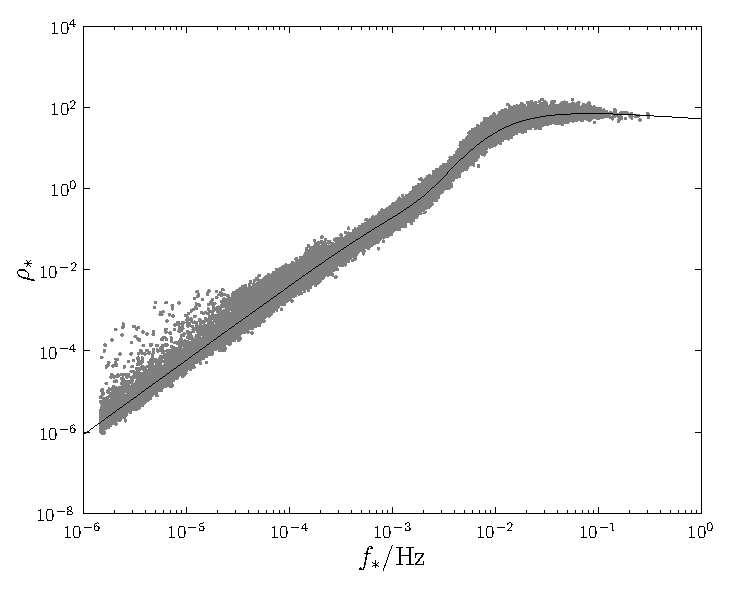
\includegraphics[width=0.43\textwidth]{Fig_SNR_scaled_fit}
 \caption{Scaled signal-to-noise ratio for EMRBs as a function of characteristic frequency.\label{fig:scaled-SNR}}
   \end{center}
\end{figure}
The curve shows that EMRB SNR does scale as expected, and $\rho_\ast$ can be describe as a one-parameter curve. There remains some scatter about this (removing the averaging over intrinsic parameters increases this to about an order of magnitude); however, it is good enough for rough calculations.

We approximate the trend with a best-fit curve
\begin{equation}
\rho_\ast = \alpha_1 f_\ast^{\beta_1} \left[1 + \left(\alpha_2 f_\ast\right)^{\beta_2}\right]\left[1 + \left(\alpha_3 f_\ast\right)^{\beta_3}\right]^{-\beta_4}.
\label{eq:scaled-SNR}
\end{equation}
To fit this, we treat the problem as if it were a likelihood maximisation, with each averaged point having a Gaussian likelihood with standard deviation defined from the scatter because of the variation in the intrinsic parameters. The optimised values for \textit{LISA} are
\begin{equation}
\begin{split}
&\alpha_1 \simeq 8.93 \times 10^4; \ \  \alpha_2 \simeq 4.68 \times 10^2; \ \  \alpha_3 \simeq 1.84 \times 10^2;\\
&\beta_1 \simeq 1.84; \ \  \beta_2 \simeq 3.23; \ \  \beta_3 \simeq 1.27; \ \  \beta_4 \simeq 4.13.
\end{split}
\end{equation}

Using our fitted trends it is possible to invert \eqnref{SNR-scaling} to find the furthest distance that bursts from an MBH of a given mass are detectable. In calculating the maximum SNR it is necessary to decide upon a minimum periapse radius. For the optimal case with a maximally rotating MBH, the innermost periapsis is $r\sub{p} = r\sub{g}$. For a non-rotating MBH, the innermost periapsis would be $r\sub{p} = 4r\sub{g}$. \Figref{detect} shows the detectability limit for $\mu = 1 M_\odot$ and $\mu = 10 M_\odot$ COs.
\begin{figure}
\begin{center}
 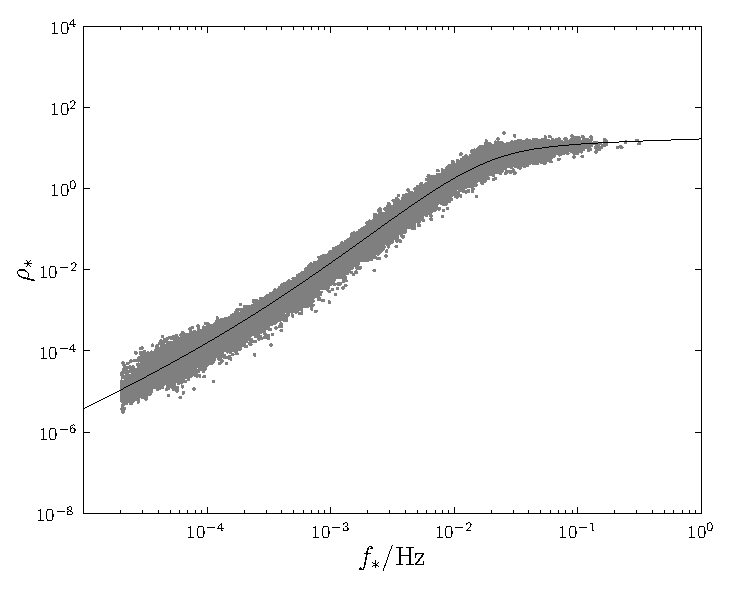
\includegraphics[width=0.43\textwidth]{Fig_SNR_scaled_fit_eLISA}
 \caption{Limit of detection for EMRBs originating from MBHs of mass $M$ and distance $R$ with CO of mass $\mu = 1 M_\odot$ () or $\mu = 10 M_\odot$. The detection threshold is assumed to be $\rho = 10$. The ... line is the limit for non-rotating MBHs, the ... line is for maximally rotating MBHs. Sources below the relevant line are potentially detectable. The trends should not be extrapolated to lower MBH masses.\label{fig:detect}}
   \end{center}
\end{figure}
The more massive COs are detectable to a greater distance, but are also the more likely sources since mass segregation ensures they are more likely to be on orbits that pass close to the MBH. Limits using periapsis of $r\sub{g}$ and $4r\sub{g}$ are shown: intermediate spin values would have limits between these two. In any case, these are strict bounds; it is unlikely that we would observe a burst from the optimal orbit. Therefore bursts from MBHs outside the curve are impossible to detect and those inside may be possible, but need not be probable, to detect.

It appears that there are potentially many galaxies which could produce observable bursts. From our sample, all could be potentially detected. Andromeda could only be detected if it had a high spin value. It is therefore less promising than the others. NGC 3489, NGC 3368 and NGC 253 lie on the boundary of detectability for non-spinning sources with a $10 M_\odot$ CO. They are therefore of marginal interest: we do not necessarily need any special requirement for the spin, but such close orbits would be infrequent. NGC 4395, NGC 4945 and Circinus are around the boundary of detectability for a $1 M_\odot$ CO. Hence we could potentially see bursts from white dwarfs as well as BHs. M32 is the best extragalactic source, lying safely within the detection limit for $1 M\odot$ COs.

We can repeat the analysis for \textit{eLISA}. The scaled SNRs are shown in \figref{scaled-SNR-eLISA}.
\begin{figure}
\begin{center}
 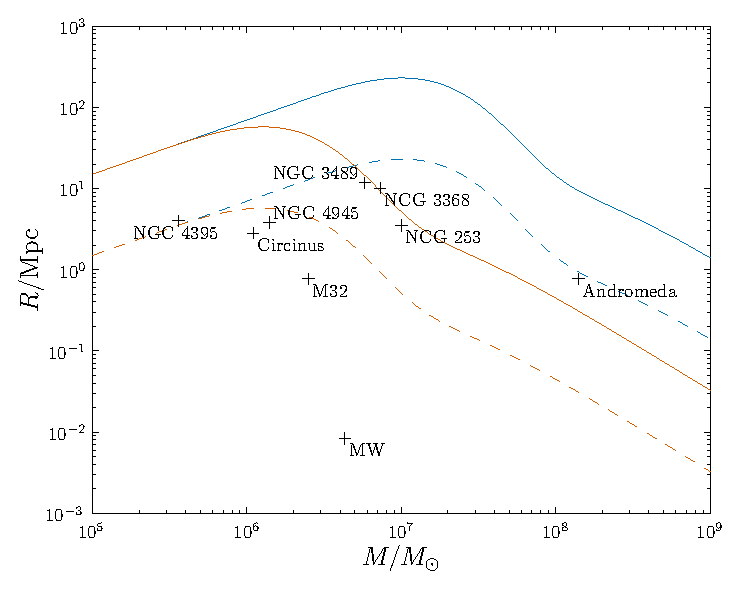
\includegraphics[width=0.43\textwidth]{Fig_M_R_detect_1}
 \caption{Scaled signal-to-noise ratio for EMRBs as a function of characteristic frequency for the \textit{eLISA} design.\label{fig:scaled-SNR-eLISA}}
   \end{center}
\end{figure}
Since Andromeda was only marginally of interest for the classic \textit{LISA} design, we did not it this time. The curve is fitted with
\begin{equation}
\begin{split}
&\alpha_1 \simeq 7.39 \times 10; \ \  \alpha_2 \simeq 4.99 \times 10^3; \ \  \alpha_3 \simeq 5.27 \times 10;\\
&\beta_1 \simeq 1.47; \ \  \beta_2 \simeq 0.85; \ \  \beta_3 \simeq 1.76; \ \  \beta_4 \simeq 1.25.
\end{split}
\end{equation}
Using this to find the detectability range results in the curves shown in \figref{detect-eLISA}.
\begin{figure}
\begin{center}
 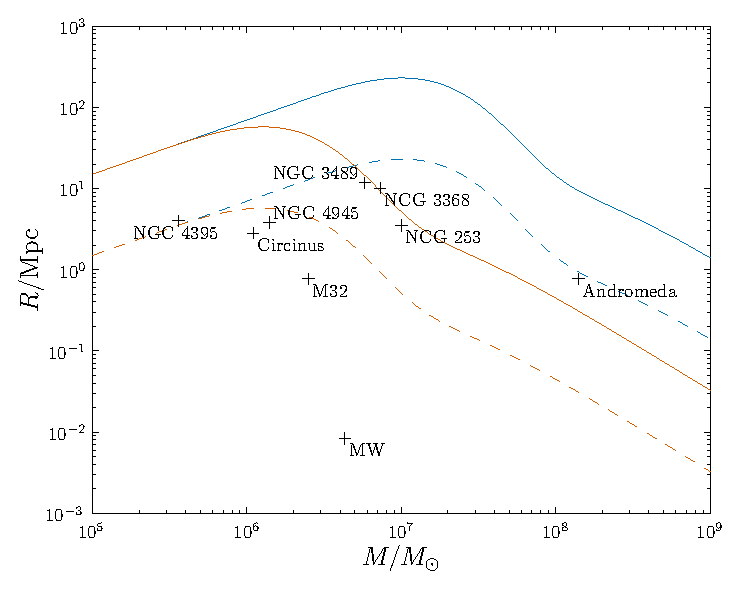
\includegraphics[width=0.43\textwidth]{Fig_M_R_detect_1}
 \caption{Limit of detection using \textit{eLISA} for EMRBs originating from MBHs of mass $M$ and distance $R$ with CO of mass $\mu = 1 M_\odot$ () or $\mu = 10 M_\odot$. The detection threshold is assumed to be $\rho = 10$. The ... line is the limit for non-rotating MBHs, the ... line is for maximally rotating MBHs. Sources below the relevant line are potentially detectable. The trends should not be extrapolated to lower MBH masses.\label{fig:detect-eLISA}}
   \end{center}
\end{figure}
The maximum distances are reduced compared to the \textit{LISA} case indicating that detectable bursts would be much rarer. There still remain a number of potential candidate galaxies. From our sample, Andromeda is on the very edge of possibility. NGC 3489, NGC 3368 and NGC 253 require a high spin, making them unlikely sources. Of the extragalactic sources, only M32 remains detectable with a $1 M_\odot$, and still it requires a non-zero spin.

Using either noise curve we see that EMRBs could potentially be seen from a range of galaxies. The Galaxy's MBH remains securely detectable in either case. M32 is the next best. MBHs with masses $\sim 10^6$--$10^7 M_\odot$ are observable to the greatest distance. We currently know of few MBHs with masses at the lower end of the spectrum, $10^5$--$10^6 M_\odot$, but these would be good potential candidates.

\section{Parameter inference}\label{sec:MCMC}

We are not only interested in if EMRBs are detectable, but also if we can extract information about their sources. The probability the burst is described by parameters $\boldsymbol{\lambda}$ is given by the posterior distribution
\begin{equation}
p(\boldsymbol{\lambda}|\boldsymbol{s}(t)) = \frac{p(\boldsymbol{s}(t)|\boldsymbol{\lambda})p(\boldsymbol{\lambda})}{p(\boldsymbol{s}(t))},
\end{equation}
where $p(\boldsymbol{s}(t)|\boldsymbol{\lambda})$ is the likelihood of the parameters, $p(\boldsymbol{\lambda})$ is the prior for the parameters, and $p(\boldsymbol{s}(t))$ is the evidence which is just a normalising factor for our purposes.

To discover if any parameters can be accurately inferred, we must characterise the form of the posterior. Markov chain Monte Carlo methods are commonly used for inference problems \citep[chapter 29]{MacKay2003}. Parameter space is explored by the construction of a chain of random samples. A new point is accepted with a rate dependent upon its probability, such that the a converged chain reflects the underlying distribution \citep{Metropolis1953,Hastings1970}. We employ the same semi-adaptive algorithm that was previously used in \citet{Berry2013}. This follows the suggestion of \citet{Haario1999} and has an initial period where the proposal distribution (used in the selection of new points) is adjusted to match the distribution of points previously accepted, before proceeding to the main phases where the proposal is kept fixed in order to be purely Markovian.

The likelihood of a set of parameters is found using \eqnref{sig_prob}:
\begin{equation}
p(\boldsymbol{s}(t)|\boldsymbol{\lambda}) \propto \exp\left[-\recip{2}\innerprod{\boldsymbol{s}-\boldsymbol{h}(\boldsymbol{\lambda})}{\boldsymbol{s}-\boldsymbol{h}(\boldsymbol{\lambda})}\right].
\label{eq:likelihood}
\end{equation}
We assume non-informative priors on the parameters to reflect a state of ignorance: we do not incorporate information we have from other measurements such that results indicate what could be leant from an EMRB alone.

\section{Conclusions}

Extreme-mass-ratio bursts have a characteristic...

The MBH in our own Galaxy is by far the best source for bursts; however, it is also possible to detect bursts from extragalactic sources. We were previously too pessimistic about this possibility \citep{Berry2013}. M32 is a promising candidate. This is good news for any space-borne GW detectors, as EMRBs can be added to the list of potential source candidates.

However, we must still be cautious: EMRBs may be rare and the event rate may prevent us from observing any over a realistic mission lifetime. In a companion paper we shall look at the expectations for bursts from our own Galaxy. Bursts from any given extragalactic source should be less common, although this may be slightly ameliorated by the larger number of potential source systems.

\section*{Acknowledgments}

The authors would like to thank Donald Lynden-Bell for useful conversations. CPLB is supported by STFC. JRG is supported by the Royal Society. The MCMC simulations were performed using the Darwin Supercomputer of the University of Cambridge High Performance Computing Service (\url{http://www.hpc.cam.ac.uk/}), provided by Dell Inc.\ using Strategic Research Infrastructure Funding from the Higher Education Funding Council for England.

\bibliographystyle{mn3e}
\bibliography{Extragalactic}

\bsp

\label{lastpage}

\end{document}
